\chapter{有质量的弱交换、虚粒子与破缺的对称性}

当我们把标准模型群解读为费米子表上的一组允许运动时，它就变得不那么神秘了。色变换在红、绿、蓝之间垂直移动。带电流弱变换在夸克和轻子二重态内部水平移动。电磁相位变换提供了第三种操作。相应的规范玻色子并不是在发现对称性之后才添加的装饰：发射一个规范玻色子，在物理上执行的正是对称性的一个生成元所描述的同一种状态改变。

这一观察引出了本讲的主要问题。弱作用顶点的耦合大小与电磁顶点相当，然而{\proseunicodefont β}衰变却比典型的强作用或电磁过程慢得多。缺失的要素是传播。在低动量下，交换一个有质量的\(W\)会在振幅中带来一个量级为\(1/m_W^2\)的因子。我们将首先在距离空间中展开这一陈述，然后在动量空间中展开，接着通过关于实粒子和虚粒子的长篇讨论追踪其后果，最后转向自发对称性破缺的第一个定性模型。

\section{从费米子表解读规范对称性}

\subsection{色作用在垂直方向}

将六种夸克味排列成三个弱族，
\begin{equation}
  (u,d),\qquad(c,s),\qquad(t,b),
\end{equation}
并给每个夸克标上红、绿或蓝的颜色标签。由此得到的夸克表有三行颜色和六列味。色\(SU(3)\)混合任意一个味列中的三个条目。例如，一个生成元可以把一个红色上夸克变成一个绿色上夸克。用粒子的语言来说，同一操作伴随着发射一个携带补偿色与反色的胶子。

同一个色变换必须作用于每一种味。把红色上夸克变成绿色上夸克的胶子，与把红色顶夸克变成绿色顶夸克的胶子是同一种类的胶子。一个真正的对称性操作不会只作用于第一代而忽略其他代。因此，色运动是垂直的且普适的：
\begin{equation}
  q_r\longleftrightarrow q_g\longleftrightarrow q_b,
  \qquad q\in\{u,d,c,s,t,b\}.
\end{equation}
它改变色，但不改变味。

这就是规范群与其规范玻色子之间的特征关系。无穷小生成元描述状态之间的变换，而相应玻色子的发射或吸收则把这些变换实现为物理过程。

\subsection{弱变换作用在水平方向}

带电流弱相互作用朝另一个方向移动。一个上型夸克可以发射一个带电流弱玻色子，变成它的下型伙伴，而不改变色：
\begin{equation}
  u_b\longrightarrow d_b+W^+.
\end{equation}
完全相同的\(W^+\)也发生在
\begin{equation}
  c_g\longrightarrow s_g+W^+,
  \qquad
  t_r\longrightarrow b_r+W^+.
\end{equation}
标签\(r,g,b\)是旁观者。胶子不会在表中水平移动，带电流的\(W\)玻色子也不会穿过色垂直移动。

再加上电磁相位对称性\(U(1)\)，在此之下每个带电的场都获得一个相位。第一遍的群结构便是
\begin{equation}
  SU(3)\times SU(2)\times U(1).
\end{equation}
叉号意味着这些是相互独立的因子：一个作用于色，一个作用于弱二重态，还有一个通过相位作用。这是有用的粗略图景，但还不是完整的电弱故事。\editorialnote{标准模型的精确规范群按惯例写作
\(SU(3)_c\times SU(2)_L\times U(1)_Y\)。弱\(SU(2)_L\)只作用于左手二重态，而最终的电磁\(U(1)_{\rm em}\)在对称性破缺之后从\(SU(2)_L\times U(1)_Y\)中涌现出来。本讲明确警告说，它对最后两个因子的第一遍认定还不完全自洽；后续各讲将补上缺失的手征结构和电弱结构。}

\subsection{同样的模式也包括轻子}

在三行颜色之下放置一行无色的轻子：
\begin{equation}
\begin{array}{c|cc|cc|cc}
 &u&d&c&s&t&b\\ \hline
Q&+\frac23&-\frac13&+\frac23&-\frac13&+\frac23&-\frac13\\
\text{lepton partner}
 &\nu_e&e^-&\nu_\mu&\mu^-&\nu_\tau&\tau^-\\
Q&0&-1&0&-1&0&-1
\end{array}
\end{equation}
在每一对相邻的条目中，电荷相差一个单位。这就是为什么同一个带电流弱玻色子能够连接\(u\)与\(d\)、\(c\)与\(s\)、\(t\)与\(b\)，以及一个带电轻子与其中微子。\(W\)顶点关心的是相应的量子数和电荷差，而不是费米子是夸克还是轻子。

\begin{figure}[htbp]
\centering
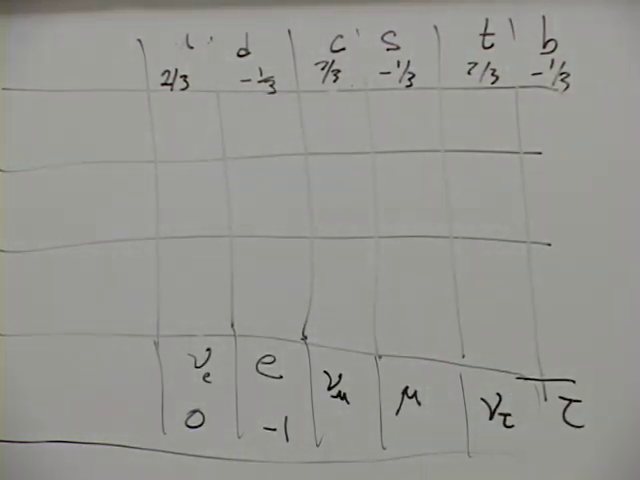
\includegraphics[width=0.88\textwidth]{lecture_06_figure_07.png}
\caption{完整的费米子表：三行夸克颜色位于无色的轻子行之上，夸克电荷和三个轻子二重态清晰可见。}
\lectureframe{00:18:55}
\end{figure}

{\proseunicodefont μ}子具有与电子相同的电荷和已知的内禀量子数，但大约重两百倍。{\proseunicodefont τ}更重。中微子质量非常小，在本讲的讨论中人们对其细节尚不清楚。这里还没有出现任何原理能够解释所观察到的族质量模式。

\begin{classroomqa}
\audiencequestion{为什么轻子、重子和介子被称为这些名字？
\lecturetimestamp{00:19:02}}
\lecturerresponse{历史上的希腊语词根大致意为轻、重和中间。这种基于质量的命名后来变得具有误导性。{\proseunicodefont μ}子曾被称为{\proseunicodefont μ}介子，因为其质量介于电子和质子质量之间，但它的相互作用表明它是轻子，与电子远比与{\proseunicodefont π}介子相似。今天，介子指夸克--反夸克强子，是玻色子；{\proseunicodefont μ}子不是介子。}
\end{classroomqa}

\section{弱相互作用的谜题}

\subsection{一个具体的带电流过程}

以中子{\proseunicodefont β}衰变作为工作图。价夸克组成为
\begin{equation}
  n=udd,\qquad p=uud.
\end{equation}
一个下夸克发生跃迁
\begin{equation}
  d\longrightarrow u+W^-,
\end{equation}
带电玻色子产生
\begin{equation}
  W^-\longrightarrow e^-+\bar\nu_e.
\end{equation}
合起来，
\begin{equation}
  n\longrightarrow p+e^-+\bar\nu_e.
\end{equation}
另外两个价夸克作为旁观者贯穿整个过程。在第一个顶点，中子变成质子；在第二个顶点，连接轻子二重态的同一种弱相互作用将\(W^-\)转化为观测到的电子和电子反中微子。

\subsection{三种耦合，三种截然不同的印象}

在QED中，电子电荷\(e\)就是顶点振幅。将其平方给出特征发射概率，常规因子收集在
\begin{equation}
  \alpha=\frac{e^2}{4\pi}\simeq\frac1{137}
\end{equation}
中（自然单位制）。强相互作用有耦合\(g_s\)，在典型强子尺度上其类似量\(\alpha_s\)可能为\(0.2\)量级。这比\(1/137\)大得多，因此当夸克被撞击时，胶子发射很常见。

令\(g_w\)表示带电弱耦合。其平方并非小得不可思议；在此处使用的量级水平上，它与电磁耦合相当。然而，自由中子等待大约十五分钟才衰变，而强衰变可能在强子穿越时间内发生。讲座中的历史估计使用较早的粗略数字十二分钟，但无论哪个数字都使同一个谜题无法回避。\editorialnote{现代自由中子平均寿命约为\(8.8\times10^2\,{\rm s}\)，主要测量方法之间持续存在实验张力。讲座中的粗略寿命被保留为教学尺度，而非精确值。}
\begin{quote}
如果\(g_w\)并非异常小，那么是什么使弱过程弱？
\end{quote}

答案不可能仅在于顶点。每个费曼图还包含传播子，即描述从一个顶点到另一个顶点的中间运动的因子。

\section{距离空间中的有质量传播子}

\subsection{顶点并非整个图}

{\proseunicodefont β}衰变图包含两个弱顶点，贡献两个\(g_w\)的幂，以及连接它们的\(W\)线。将位置空间传播子记为\(\Delta(x-y)\)，其中\(x\)是发射事件，\(y\)是吸收或转化事件。它是与在这些事件之间传递场扰动相关联的振幅核。

精确的相对论传播子包含比我们所需更多的结构。其重要的定性特征是对质量的依赖。在短类空间隔下，它具有幂律奇异性，示意为
\begin{equation}
  \Delta(d)\sim\frac1{d^2}.
\end{equation}
无质量场保留幂律尾部。相比之下，有质量场一旦间隔变得大于其康普顿尺度，就受到指数抑制。因此曲线急剧向下弯折。

\subsection{自然单位制定位弯折}

设
\begin{equation}
  c=\hbar=1.
\end{equation}
则
\begin{equation}
  [m]=[E]=[p]=L^{-1}.
\end{equation}
熟悉的关系解释了每个等式：\(E=mc^2\)将质量与能量等同，而\(p\,x\)具有\(\hbar\)的量纲，因此动量和距离具有相反的单位。因此，唯一能由质量\(m\)构成的长度是
\begin{equation}
  d_m\sim\frac1m.
\end{equation}
恢复常数给出
\begin{equation}
  d_m\sim\frac{\hbar}{mc},
\end{equation}
即康普顿波长。较重的交换粒子具有较短的有效力程。

\begin{figure}[htbp]
\centering
\includegraphics[width=0.78\textwidth]{lecture_06_figure_02.png}
\caption{自然单位制量纲与定性传播子衰减。黑色曲线继续以幂律尾部延伸；红色有质量曲线在反质量尺度附近向下转折。}
\lectureframe{00:27:19}
\end{figure}

\begin{figure}[htbp]
\centering
\begin{tikzpicture}[x=1.0cm,y=0.9cm]
  \draw[->] (0,0) -- (7,0) node[right] {$d$};
  \draw[->] (0,0) -- (0,5) node[above] {$|\Delta(d)|$};
  \draw[thick]
    plot[smooth] coordinates {(0.45,4.5) (0.9,3.3) (1.6,2.5)
      (2.5,1.9) (3.7,1.45) (5.1,1.12) (6.4,0.9)};
  \draw[thick,red]
    plot[smooth] coordinates {(0.45,4.5) (0.9,3.3) (1.6,2.5)
      (2.5,1.9) (3.2,1.55) (3.7,0.95) (4.2,0.36) (4.8,0.1)};
  \draw[dashed] (3.4,0) -- (3.4,1.4);
  \node at (5.7,1.4) {$m=0$};
  \node[red] at (4.75,0.72) {$m>0$};
  \node[below] at (3.4,0) {$d\sim m^{-1}$};
\end{tikzpicture}
\caption{黑板论证的清晰示意图。它不是四维传播子的精确公式；它分离出质量控制的区间。}
\end{figure}

\begin{classroomqa}
\audiencequestion{纵轴上画的是什么？
\lecturetimestamp{00:28:30}}
\lecturerresponse{传播子的大小，记作\(\Delta\)。在完整的振幅、外部态和相空间因子都包含进来之后，它的平方对概率有贡献。该图意在表明，大质量交换在长距离上的振幅会迅速关断。\editorialnote{传播子本身并不是一个可直接测量的、对应于粒子沿经典路径运动的概率振幅。讲义中的说法是一种有用的量级估计：传播子只是完整散射或衰变振幅中的一个因子。}}
\end{classroomqa}

\section{傅里叶变换与费米极限}

\subsection{实验给定的是动量}

实验通常测量的是外部动量，而不是内部线开始和结束的两个时空点。在{\proseunicodefont β}衰变中，\(W\)所携带的动量由中子与质子动量之差推断出来，它等于电子与反中微子的总动量。位置空间传播子与动量空间传播子通过傅里叶变换相联系。
\begin{equation}
  k=p_n-p_p=p_e+p_{\bar\nu_e}.
\end{equation}

在板书上所用的正分母约定下，
\begin{equation}
  \widetilde{\Delta}_W(k)=\frac1{k^2+m_W^2},
  \qquad
  \widetilde{\Delta}_\gamma(k)=\frac1{k^2}.
\end{equation}
无质量光子传播子在小动量转移时变得很大。有质量的\(W\)传播子永远不会超过\(1/m_W^2\)量级的尺度。对于{\proseunicodefont β}衰变，
\begin{equation}
  |k^2|\ll m_W^2,
\end{equation}
因此\(k^2\)的细节可以忽略，并且
\begin{equation}
  \widetilde{\Delta}_W(k)\simeq\frac1{m_W^2}.
\end{equation}

\begin{classroomqa}
\audiencequestion{相对论性的\(k^2\)在能量与空间动量之间是否应包含一个负号？
\lecturetimestamp{00:35:11}}
\lecturerresponse{是的。在主要为负号的闵可夫斯基度规下，
\(k^2=(k^0)^2-\boldsymbol{k}^2\)，而标量分母按惯例为
\(k^2-m_W^2+i\epsilon\)。板书使用的是等价的、正的空间类或欧几里得大小。在低能{\proseunicodefont β}衰变中，转移的四动量与\(m_W\)相比极小，因此两种记号给出相同的\(1/m_W^2\)压低，至多相差振幅中一个无关紧要的符号。}
\end{classroomqa}

\subsection{低能振幅}

两个弱顶点和一个传播子给出
\begin{align}
  \mathcal A_{\rm weak}
  &\sim g_w\,\widetilde{\Delta}_W(k)\,g_w\\
  &\sim\frac{g_w^2}{k^2+m_W^2}
  \simeq\frac{g_w^2}{m_W^2}.
\end{align}
将振幅平方后产生特征性的压低
\begin{equation}
  |\mathcal A_{\rm weak}|^2
  \sim\frac{g_w^4}{m_W^4},
\end{equation}
这是在包含特定衰变所对应的运动学和相空间因子之前。弱相互作用在核能标下之所以弱，并不是因为它的基本规范耦合小得荒谬，而是因为它的媒介粒子很重。

\begin{figure}[htbp]
\centering
\includegraphics[width=0.86\textwidth]{lecture_06_figure_03.png}
\caption{中子--质子的弱过程以及内部线所携带的动量转移，正如在确定传播子符号时所讨论的那样。}
\lectureframe{00:35:40}
\end{figure}

\begin{figure}[htbp]
\centering
\includegraphics[width=0.84\textwidth]{lecture_06_figure_04.png}
\caption{{\proseunicodefont β}衰变拓扑结构，旁边是方框中的低能估计\(g_w^2/m_W^2\)。}
\lectureframe{00:37:25}
\end{figure}

在数值上，按本讲义的精度，\(m_W\)大约是质子质量的一百倍。振幅中的一个\(m_W^{-2}\)因子在速率中变成\(m_W^{-4}\)，因此即使耦合具有普通规范理论的量级，也会产生非常长的寿命。

\begin{classroomqa}
\audiencequestion{我们说的是百万分之一的压低还是十亿分之一的压低，以及\(W\)质量最初是如何知道的？
\lecturetimestamp{00:38:11}}
\lecturerresponse{讲义中的粗略计数指向低能弱概率相对于未压低的强子过程具有十亿量级的小量。历史上，低能实验并没有分别测量\(g_w\)和\(m_W\)。它们测量的是小组合
\(g_w^2/m_W^2\)，称为费米常数。一旦规范耦合与电弱理论联系起来，该组合就预言了一个非常重的媒介粒子；后来的加速器直接产生了\(W\)并测量了它的质量。}
\end{classroomqa}

在远低于\(m_W\)的动量下，每个实验看到的几乎是同一个常数：
\begin{equation}
  G_F\sim\frac{g_w^2}{m_W^2}.
\end{equation}
这就是为什么费米能在1930年代把{\proseunicodefont β}衰变描述为点状四费米子相互作用，远在媒介粒子被观测到之前。随着碰撞能量提高，实验开始对传播子中隐藏的动量依赖性敏感，从而证实该有效常数是大质量交换在低能下的影子。\editorialnote{在树图阶采用标准电弱归一化时，
\[
  \frac{G_F}{\sqrt2}=\frac{g^2}{8m_W^2}.
\]
讲义有意省略了数值因子和旋量因子，只保留标度关系\(G_F\sim g_w^2/m_W^2\)。\(W\)和\(Z\)于1983年在CERN被直接发现；讲义中顺带提到的1970年代中后期对于直接观测来说太早了。}

历史上，弱相互作用可能由一种重粒子传递的想法出现于二十世纪中叶；讲座提到朱利安·施温格是探索这一可能性的理论家之一，并指出字母\(W\)很可能代表弱。低能数据早已暗示，这种传递粒子在核尺度上必须极其重，远在加速器拥有足够能量将其作为真实粒子产生之前就是如此。

\subsection{对一个速率的三种独立控制}

一个关于核束缚的课堂提问区分了对跃迁的三种逻辑上不同的控制：
\begin{enumerate}
  \item 顶点耦合常数；
  \item 传播子，包括质量和动量依赖；
  \item 可用的初态到末态能量与相空间。
\end{enumerate}
束缚可以关闭一个衰变道，因为末态的能量会大于初态。这是一种运动学禁止，而不是对\(g_w\)的进一步压低，也不是\(m_W\)的改变。当一个道仍然开放但可用能量很少时，其相空间仍可能被强烈压低。

\begin{classroomqa}
\audiencequestion{附近质子的场或束缚是否会通过同样的传播子机制压低{\proseunicodefont β}衰变？
\lecturetimestamp{00:41:13}}
\lecturerresponse{在所讨论的例子中不会。束缚之所以重要，是因为它改变了初态和末态核态的能量。如果末态在能量上不可及，过程就不能发生。耦合、传播子和可用能量是三种彼此独立的要素。}
\end{classroomqa}

\begin{classroomqa}
\audiencequestion{耦合常数真的是常数吗？
\lecturetimestamp{00:42:55}}
\lecturerresponse{只在固定标度下如此。量子修正使有效耦合随动量或距离跑动。目前的论证是在与该过程相关的标度上处理每个耦合；标度依赖将在后面展开。}
\end{classroomqa}

\section{不放弃守恒律的虚交换}

\subsection{为什么重粒子线可以出现}

普通中子衰变没有足够能量产生一个自由的、在壳的\(W\)。图中的\(W\)是内部的且离壳。讲座用传统的能量--时间估计引入这一事实：
\begin{equation}
  \Delta E\,\Delta t\lesssim\hbar:
\end{equation}
一个经典能量看起来差了\(\Delta E\)的中间构型，只能在量级为
\(\hbar/\Delta E\)的时间内贡献。

隧穿类比使所要表达的图像变得生动。把一个{\proseunicodefont α}粒子放入核势阱中。它的能量低于势垒顶部，因此经典上它不能逃逸。量子力学上，波函数延伸到势垒之中，粒子可以在远侧某点出现，并具有与初始相同的总能量。如果我们试图把势垒内部描述为普通的经典轨迹，势能似乎太大，而动能将不得不为负。那幅失败的经典图像，类似于试图把内部\(W\)看作真实粒子。

\begin{figure}[htbp]
\centering
\includegraphics[width=0.78\textwidth]{lecture_06_figure_06.png}
\caption{隧穿类比：初始点和远侧斜坡上标记的点具有相等的总能量，而介于其间的势垒在经典上是禁戒的。}
\lectureframe{00:46:00}
\end{figure}

\begin{figure}[htbp]
\centering
\begin{tikzpicture}[x=1.0cm,y=0.9cm]
  \draw[->] (0,0) -- (7,0) node[right] {$x$};
  \draw[->] (0,0) -- (0,4.8) node[above] {$V(x)$};
  \draw[thick]
    plot[smooth] coordinates {(0.3,1.4) (1.0,0.7) (1.7,0.55)
      (2.1,0.9) (3.2,3.9) (4.2,2.1) (5.0,0.75) (6.6,0.18)};
  \draw[dashed] (1.7,0.75) -- (5.0,0.75);
  \fill (1.7,0.75) circle (0.06);
  \fill (5.0,0.75) circle (0.06);
  \node at (3.35,0.35) {$\Delta E\,\Delta t\lesssim\hbar$};
\end{tikzpicture}
\caption{势垒与等能量点的一个可读重建。}
\end{figure}

在{\proseunicodefont β}衰变图像中，中子可以涨落为质子加一个内部\(W^-\)，但重粒子线必须很快被移除。它可能被重新吸收，恢复中子；也可能终止于第二个顶点，并产生轻得多的电子和反中微子。完整的初态和末态能量一致。\editorialnote{能量和动量在每个费曼顶点都守恒。虚粒子并不是真的借来能量再稍后偿还。精确的陈述是，内线要对四动量积分，而这些四动量不必满足真实粒子的质壳关系\(k^2=m_W^2\)。不确定性原理和隧穿语言被保留下来，因为这是讲座的解释路径，但离壳陈述才是现代量子场论的表述。}

\subsection{真实W玻色子}

能量足够高的加速器可以产生一个真实的\(W\)。此时它具有自身的固有寿命，与那条虚粒子线假想的不确定时间无关。一个被加速的真实\(W\)在实验室中会因普通的相对论时间膨胀而存活更久。在静止的\(W\)的两体轻子衰变中，\begin{equation}
  W^-\longrightarrow e^-+\bar\nu_e,
\end{equation}电子和反中微子携带很大的、几乎背对背的动能，各自量级为\(m_W/2\)。静止能量并没有消失；它变成了末态能量。{\proseunicodefont μ}子和{\proseunicodefont τ}子通道以及夸克通道也同样可用。

\begin{classroomqa}
\audiencequestion{一个真实的\(W\)能存活多久，它的寿命能否由同一个耦合计算出来？
\lecturetimestamp{00:49:49}}
\lecturerresponse{可以。人们计算每个允许的衰变振幅，将其平方，对末态相空间积分，再把各分宽度求和。总宽度的倒数给出寿命。转录中口述的数值估计有误，但定性的要点是：固有寿命极短，而运动中的\(W\)按通常方式发生时间膨胀。\editorialnote{利用测得的宽度\(\Gamma_W\simeq2.1\,{\rm GeV}\)可得
\(\tau_W=\hbar/\Gamma_W\simeq3.2\times10^{-25}\,{\rm s}\)。这个现代数值解决了被损坏的数值交流，而不把它归因于讲座。}}
\end{classroomqa}

\begin{classroomqa}
\audiencequestion{振幅的平方如何变成一个速率，进而变成寿命？
\lecturetimestamp{00:50:52}}
\lecturerresponse{将矩阵元的平方与可用末态密度、守恒{\proseunicodefont δ}函数以及归一化因子结合起来，得到单位时间的概率，即衰变宽度\(\Gamma\)。在\(\hbar=1\)的单位制下，存活概率为\(e^{-\Gamma t}\)，因此\(\tau=1/\Gamma\)，或者恢复单位后为\(\tau=\hbar/\Gamma\)。因此，小的弱宽度意味着长的弱寿命。}
\end{classroomqa}

\begin{classroomqa}
\audiencequestion{能否给穿越势垒的隧穿粒子赋予一个速度？
\lecturetimestamp{00:52:42}}
\lecturerresponse{可以用推断的距离除以推断的穿越时间，但那个量不应被解释为经典粒子的速度或信号的速度。试图测量势垒内部的轨迹会改变状态，并破坏原来的隧穿实验。}
\end{classroomqa}

\section{观测一个虚粒子意味着什么？}

\subsection{外线粒子与内线}

真实粒子是可以在相互作用区域之外制备或探测到的入射和出射渐近态。虚粒子是振幅的微扰表示中的内线。它们不是额外的隐藏探测器轨迹。

\begin{classroomqa}
\audiencequestion{真实粒子与虚粒子之间的区别是否有清晰的定义？
\lecturetimestamp{00:55:05}}
\lecturerresponse{真实粒子是进入或离开相互作用区域的外线在壳态。虚粒子是费曼图中的内线离壳线。后者是数学展开的一部分，而不是独立观测到的客体。}
\end{classroomqa}

要分辨一个仅持续\(\Delta t\)的过程，探针需要量级为\(1/\Delta t\)的频率，因而需要量级为\(\hbar/\Delta t\)的能量。一个足够锐利、能分辨高势垒下方{\proseunicodefont α}粒子的光子，可以提供把它提升到势垒区域所需的能量。同样，一个能量足够高、能分辨短寿命内部\(W\)的探针，可以产生一个真实的\(W\)。这种试图观测把原来的过程变成了另一个实验。

讲座把这表述为一种反复出现的量子力学挫败：检查那个被禁止的中间图像所需的干预，恰恰提供了使这个看似被禁止的组态成为真实的能量。

\subsection{质子的涨落}

在微扰论中，质子态包含诸如
\begin{equation}
  p\longleftrightarrow n+W^+,
\end{equation}
等组态的振幅，而中子同样有
\begin{equation}
  n\longleftrightarrow p+W^-.
\end{equation}
如果没有其他相互作用介入，内部玻色子会被重新吸收。而硬探针则可以在出射粒子中留下一个\(W\)。人们可以把这一行为称为敲出一个涨落，或产生一个\(W\)。说法不同；可测量的陈述是同一个末态振幅。

\begin{classroomqa}
\audiencequestion{当一个硬探针产生一个出射的\(W\)时，它是敲出了一个已经在那里的粒子，还是创造了一个新粒子？
\lecturetimestamp{01:01:20}}
\lecturerresponse{两种图像都可以组织数学。一种时间有序的描述说，质子涨落为\(n+W^+\)，探针在重新吸收之前移走了中子；另一种说，碰撞产生了末态\(W\)。不变的是所观测末态的计算概率，而不是关于测量之前存在什么的唯一经典故事。}
\end{classroomqa}

提高碰撞能量并不会揭示出原本隐藏在靶内部的一批固定对象。它会打开许多可能的末态：一个\(W\)、若干玻色子、夸克喷注、强子，以及由守恒量子数所允许的其他粒子。即使是对一个基本场进行足够剧烈的撞击，也能产生质子以及许多其他复合对象。产生出来的东西不必事先作为组成部分存在。讲座把这一点推向了滑稽的极端：如果能量和量子数允许，那么即便是桌子、椅子或一个氢原子，作为极其不可能但逻辑上并非被排除的末态排列，也并非不可能。这个玩笑承载着一个严肃的警告：不要用对碰撞碎片的朴素清点来定义基本性。

\subsection{真空涨落与温度}

附着在质子上的涨落与真空图并不相同。前者是相互作用质子态的一个组成部分；真空涨落没有外部的质子线。在两种情况下，一个能量足够高的探针都可能产生与某个允许末态相对应的实粒子。例如，当质心能量超过阈值时，两个高能光子可以产生一个电子--正电子对。

\begin{classroomqa}
\audiencequestion{这些反应依赖于温度吗？
\lecturetimestamp{01:05:17}}
\lecturerresponse{基本振幅并不需要热浴。温度在统计上起作用：高温系统包含许多具有高动能的粒子，因此跨越阈值的碰撞会变得常见。加热一个包含束缚{\proseunicodefont α}粒子的系统，除了量子隧穿之外，还可能提供足够的能量使其越过势垒逃逸。少数孤立的 energetic 粒子构成一束束流；许多按热分布的高能粒子构成一个热浴。}
\end{classroomqa}

\begin{classroomqa}
\audiencequestion{在质子涨落中发射的\(W\)是真空的涨落吗？
\lecturetimestamp{01:06:56}}
\lecturerresponse{不是。\(p\leftrightarrow n+W^+\)中的内部\(W\)是相互作用质子态的涨落。没有外部质子的闭合虚过程是真空涨落。它们遵循相同的场论规则，但属于不同的振幅。}
\end{classroomqa}

\begin{classroomqa}
\audiencequestion{为什么在轻子\(W\)顶点处需要反中微子？
\lecturetimestamp{01:08:51}}
\lecturerresponse{它提供了守恒的轻子量子数，并且是连接\(e\)、\(\nu_e\)和\(W\)的基本带电流顶点的一部分。横杠把出射的电子反中微子与中微子区分开来。}
\end{classroomqa}

\section{能量转换能被推到多远？}

接下来这节课把能量可以产生粒子这一规则推向一个刻意荒谬的极限。一颗咖啡豆能变成一块巧克力蛋糕吗？并不存在那种实际过程，但相对论量子理论并不强加一条规则，要求末态物质必须与初始对象相似。它要求足够的能量、正确的守恒荷以及非零振幅。一千克所具有的能量量级为
\begin{equation}
  Mc^2\sim9\times10^{16}\ {\rm J},
\end{equation}
因此，任何组装出某个千克尺度特定对象的微观碰撞，都将超出极其不可能的范围。

普朗克质量，
\begin{equation}
  m_{\rm P}=\sqrt{\frac{\hbar c}{G}}
  \simeq2.2\times10^{-5}\ {\rm g},
\end{equation}
并不是可能的最大质量。它是当量子被局域在其康普顿波长上时引力变得很强的尺度。一千克大约包含\(5\times10^7\)个普朗克质量。

\begin{classroomqa}
\audiencequestion{如果碰撞超过普朗克尺度，椅子或行星等任意重的物体能够出现吗？
\lecturetimestamp{01:10:37}}
\lecturerresponse{在集中于小区域的跨普朗克质心能量下，引力坍缩是压倒性地自然的结果：一个黑洞。一个高度有序的宏观对象将是一种极其罕见的涨落。讲座援引了时间反演：因为椅子可以落入黑洞，所以反向振幅并非严格为零。它的概率被一个巨大的熵因子所压低，因此不能把可能性与实际可能性混为一谈。}
\end{classroomqa}

这次离题强化了先前的警告。量子场论预言的是指定初态与末态之间的振幅。那种认为每个产物在碰撞前都字面地包含在靶中的生动说法，并不是这一预言的一部分。

\section{玻色子、它们的相互作用及其统计}

\subsection{光子可以散射}

是玻色子并不意味着不参与相互作用。玻色子或费米子规定的是交换统计；相互作用顶点则是另外的动力学事实。经典光束通常彼此穿过，因为QED没有树级的四光子顶点，而低能光子--光子散射极其微小。尽管如此，两个光子仍可通过虚电子--正电子圈发生相互作用：
\begin{equation}
  \gamma+\gamma
  \longrightarrow(e^-e^+)_{\rm virtual}
  \longrightarrow\gamma+\gamma.
\end{equation}
当质心能量足够高时，它们反而可能产生一对实粒子，
\begin{equation}
  \gamma+\gamma\longrightarrow e^-+e^+.
\end{equation}
光学光子的能量为几个电子伏特，而电子对阈值约为\(2m_e c^2\approx1.02\,{\rm MeV}\)。因此，在通常的光学能量下，该虚过程受到强烈压低，这就是交叉光束看起来彼此互不察觉的原因。

\begin{classroomqa}
\audiencequestion{虚\(W\)玻色子仅仅因为它们是玻色子就与其他玻色子相互作用吗？
\lecturetimestamp{01:12:47}}
\lecturerresponse{它们可以相互作用，但并非仅仅因为它们服从玻色统计。规范顶点决定动力学相互作用。统计所决定的，是当全同粒子被交换时多粒子振幅如何表现。光子通过带电虚粒子发生微弱相互作用，而电弱理论还包含直接的非阿贝尔\(W\)玻色子自相互作用。}
\end{classroomqa}

\subsection{玻色增强不是一种力}

当若干全同粒子占据邻近的量子态时，费米子统计与玻色子统计的差别就变得显著。玻色子倾向于多重占据；费米子则排除全同占据。在典型的高能碰撞中，粒子飞入彼此分离得很开的动量态，因此这种统计效应可能不如在激光或凝聚体中那样明显。

原则上，\(W\)玻色子具有同样的玻色增强。讲座中开玩笑说，可以想象一个使\(W\)玻色子产生激光的系统。它们巨大的质量和极短的寿命使这样的装置极不切实际，但其统计确实是玻色统计。

\begin{classroomqa}
\audiencequestion{质子或中子是什么颜色？
\lecturetimestamp{01:18:41}}
\lecturerresponse{一个物理强子是一个色单态，常被称为无色或白色。简写说法称，一个重子包含一个红夸克、一个绿夸克和一个蓝夸克。更准确地说，它的色波函数是反对称叠加
\[
  |{\rm singlet}\rangle
  =\frac1{\sqrt6}\epsilon_{abc}|q^a q^b q^c\rangle,
\]
而不是对每个被命名的夸克永久指定某种颜色的经典指派。}
\end{classroomqa}

\begin{classroomqa}
\audiencequestion{玻色凝聚会进入本课程吗？
\lecturetimestamp{01:19:25}}
\lecturerresponse{会，通过希格斯现象。真空中处处非零的希格斯场在重要方面类似于玻色凝聚体。这一类比将在引入自发对称性破缺之后展开。\editorialnote{希格斯真空期望值并不是字面意义上由在壳希格斯粒子占据一个态所组成的普通气体。凝聚是对相干玻色场和选定真空的一种富有启发性的类比，而不是完整的微观等同。}}
\end{classroomqa}

\section{缺失的中性弱玻色子}

现在回到群表。如果水平方向的弱对称是\(SU(2)\)，那么它有
\begin{equation}
  \dim SU(2)=3
\end{equation}
个生成元，因此有三个规范场。带电组合\(W^+\)和\(W^-\)只解释了其中两个。还需要第三个中性场。它与观测到的\(Z\)玻色子密切相关，但并不简单地就是光子。精确的中性组合同时涉及第三个\(SU(2)_L\)场和\(U(1)_Y\)场。这种混合，连同电荷的正确定义，被有意推迟到下一讲。

\section{自发对称性破缺}

\subsection{对称的选择可能具有不稳定的犹豫不决}

想象一张圆形餐桌，每个座位左边放一件餐具，右边放一件餐具。在任何人动作之前，左和右是等价的。一旦一位客人伸手向右，邻近的每个选择都被迫随之确定，整张桌子便稳定为右手安排。规则是对称的，但实际实现的构型选择了两种可能性之一。这个故事只是一个类比，但它分离出了我们所需要的组合：对称性、多个等价结果，以及一种不稳定性，使任意小的扰动能够在全局上选定一个结果。

\subsection{正面--反面的点阵}

为了得到更简洁的模型，在点阵的每个格点上放置一个二态变量 \(s_i=\pm1\)。称 \(+1\) 为正面，\(-1\) 为反面。让相邻格点倾向于对齐：
\begin{equation}
  H=-J\sum_{\langle ij\rangle}s_i s_j,
  \qquad J>0.
\end{equation}
平行相邻格点比反平行相邻格点贡献更低的能量。因此存在两个简并基态，
\begin{equation}
\begin{aligned}
  s_i&=+1\quad\text{for every }i,
  \\
  s_i&=-1\quad\text{for every }i.
\end{aligned}
\end{equation}
哈密顿量在全局翻转 \(s_i\to-s_i\) 下不变，但任一选定的基态则不然。

现在把某个非常遥远的边界自旋固定为正面。在普通的短程系统中，我们或许会预期一个远处的自由度对这里没有影响。然而在有序相中，该边界条件会选出全正面的真空。一旦选定，正面海洋中的单个反面就会因为与相邻格点不一致而付出能量代价。局域激发是相对于所选基态定义的，尽管底层方程仍保留正面--反面的对称性。

\subsection{显式破缺与畴壁}

显式破缺会加入一个局域偏置，
\begin{equation}
  H_{\rm explicit}
  =-J\sum_{\langle ij\rangle}s_i s_j-h\sum_i s_i,
  \qquad h\ne0.
\end{equation}
于是即使在单个孤立格点上，正面与反面也不具有相等的能量，并且只有一个优先真空。在自发破缺中 \(h=0\)：局域规则是对称的，两个真空仍然简并，但系统占据其中之一。

反之，坚持最左边界全为正面、最右边界全为反面。最低能量构型必须在两个真空之间插值。这个界面就是畴壁。

\begin{figure}[htbp]
\centering
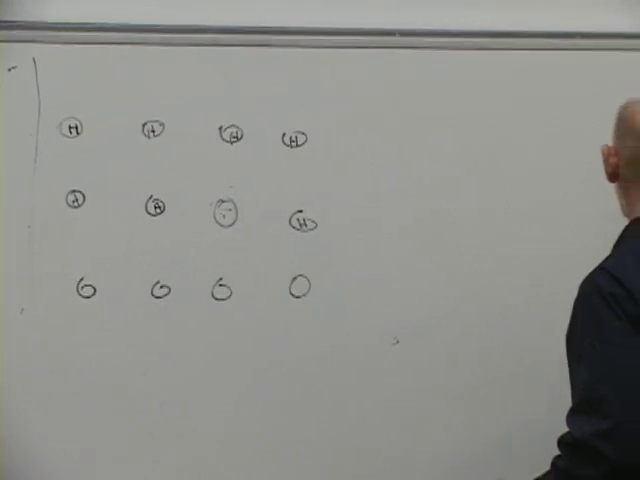
\includegraphics[width=0.9\textwidth]{lecture_06_figure_08.png}
\caption{被虚线畴壁分隔的正面--反面点阵。相反的边界条件迫使系统在两个简并有序态之间包含一个界面。}
\lectureframe{01:30:35}
\end{figure}

\begin{classroomqa}
\audiencequestion{自发对称破缺与普通的显式对称破缺有何区别？
\lecturetimestamp{01:28:36}}
\lecturerresponse{在显式破缺中，局域哈密顿量已经赋予正面和反面不同的能量，因此不存在一对由对称性联系的基态。在自发破缺中，方程仍保留对称性，真空是简并的，而边界条件或任意小的扰动会选出其中一个。在不同真空之间插值的畴壁的可能性，是后一种情形的判据。}
\end{classroomqa}

这个模型是刻意朴素的，但它包含了将被转移到希格斯场的关键逻辑：一个对称的理论、一个不稳定或简并的真空结构、一个被选定的基态，以及由该选择所决定的物理后果。

\section{本讲留给我们的问题}

费米子表把标准模型群变成了一组物理方向。颜色 \(SU(3)\) 在红、绿、蓝之间竖直移动；带电流弱变换在夸克和轻子二重态之间水平移动；一个相位对称性提供了初步的 \(U(1)\) 因子。规范玻色子的发射把这些群变换实现为相互作用。

于是{\proseunicodefont β}衰变的微弱并非归因于异常小的 \(g_w\)，而是归因于重媒介子。在距离空间中，质量在康普顿尺度 \(\hbar/(m_Wc)\) 之外截断传播子。在动量空间中，
\begin{equation}
  \mathcal A_{\rm weak}
  \sim\frac{g_w^2}{k^2+m_W^2}
  \simeq\frac{g_w^2}{m_W^2}
\end{equation}
在核动量下成立。早期的低能实验把这个组合测量为费米常数。

扩展的课堂讨论澄清了这个公式意味着什么、不意味着什么。内部 \(W\) 线是虚的且离壳；能量--动量仍然守恒。足够硬的探针可以产生一个实的 \(W\)，但那时它已经产生了一个不同的末态过程。碰撞产物并不是预先存在的组分的字面清单。温度改变高能入射粒子的布居，光子可以通过带电虚粒子相互作用，而玻色统计与动力学力是不同的。

最后，\(SU(2)\) 需要一个与 \(Z\) 相关的缺失中性规范场，而正面--反面点阵提供了自发对称破缺的第一个模型。下一步是把这两条未完成的线索结合起来：电弱混合与希格斯机制。
